\documentclass{article}
\usepackage{graphicx}
\usepackage{array}
\usepackage{tabularx}
\graphicspath{ {images/} }
\usepackage[utf8]{inputenc}
\newcolumntype{Y}{|>{\centering\arraybackslash}X}
\title{TAMIL TEXT TO ENGLISH EMOTIONAL SPEECH CONVERSION WITH UNL FOR TRANSLATION
}
\author{B.ARCHANA - 2011103505 \\ M.R.SIVA - 2011103536\\R.JAYAVASANTH-2011103562\\\\\\\\Project Guide : Dr. Rajeswari Sridhar\\Asst. Professor (Sr. Grade)\\Department of Computer Science and Engineering,\\
Anna University, Chennai - 25}
\usepackage{geometry} 
\geometry{ 
a4paper, 
total={210mm,297mm}, 
left=30mm, 
right=30mm, 
top=30mm, 
bottom=20mm, 
}

\begin{document}

\maketitle

\section{Introduction}\large
This project in the field of Natural Language Processing aims at
translating an input Tamil sentence into an equivalent spoken English
translation of the sentence. This brings together two major domains in
NLP,i.e, machine translation and TTS(Text to Speech). Natural
Language Processing is the field of computer science that deals with
interactions between computer and human languages. One of the aim
of NLP is ”Natural Language Understanding”, i.e., to enable computers
to derive meaning from human language input. Computational
linguistics is a sub domain under NLP, which focuses specifically on
language related work such as language modelling, representation.
Machine Translation is one such field of computational linguistics.
Machine Translation involves the development of software for
translation of given text from a source language to the target
language.
\section{Problem Statement}\large
Given a Tamil sentence as input, the project will translate it into its corresponding English sentence with no loss in meaning while preserving the semantic structure of English.The translated sentence would be voiced over with a humanised robotic voice. Given a batch of sentences ( document input ), each sentence would be processed and translated and synthesised into speech.
\section{Project Description}\large
The first phase of the project i.e,conversion of Tamil input text
into English is done by converting Tamil text into the Universal
Networking Language representation and then converting from UNL into
the equivalent English form. Here UNL is used as the pivot language in
between the Tamil and English languages. Since UNL is
language-independent, it offers a very flexible platform for the
representation of knowledge and thus gives great scope for research,
in conjunction with the rich language of Tamil, that we have
undertaken in our project.
The second phase of our project takes the converted English text and
processes it with a Text-To-Speech Engine, to convert it into speech.
This TTS system is modified at signal level so as to incorporate
emotion, to make the robotic speech more humanised. The given text
is transformed into speech with the necessary prosody,stress and
intonation marked so as to add emotion to the text.
\section{Literature Survey}\large
\begin{enumerate}
\item \textbf{Dhanalakshmi V., Anand kumar M., Soman K. P. and Rajendran S., \textit{"Postagger and Chunker for Tamil Language"}, Proceedings of the 8th Tamil Internet Conference, Cologne, Germany, 2009.}
\\This paper makes use of machine learning techniques to carry out POS tagging of tamil sentences. A custom tagset was developed to annotate the Tamil corpus for training and testing. Customised tagset reduces time and complexity increasing tagging accuracy.

\item \textbf{Rajeswari Sridhar, Sugadev C, Mani Murugesan P, Vignesh N T,  \textit{"A hybrid approach to Tamil Morphological generation"}, 13th International Tamil Internet Conference, pp 101- 105, Pondicherry, 2014.}
\\adgbs

\item \textbf{T.Dhanabalan, K.Saravanan, T.V.Geetha,\textit{ “Tamil to UNL EnConverter”.}}
\\This paper defines all the possible relations that can exist between two UNL nodes based on the suffixes of words. It handles the construction of Simple Nodes only.

\item \textbf{J Balaji, T V Geetha, RanjaniParthasarathi,  MadhanKarky, \textit{“Morpho-Semantic Features for Rule-based Tamil Enconversion”}} 
\\This paper elaborates on the rules for forming UNL graphs from suffixes. However this paper does not consider the relations associated with complex and compound tamil Sentences.

\item \textbf{Balaji J, Geetha T V, RanjaniParthasarathi, \textit{“Semantic Parsing of Tamil Sentences.”}}
\\This paper talks about identifying the subgraphs in a sentence using certain inflictions that corresponds to pos,mod relations.

\item  \textbf{Tristan Bowles,SandraPauletto,  \textit{“Emotions in the Voice Humanising a Robotic Voice”}, In Proceedings of the 7th Sound and Music Computing Conference, Barcelona, Spain, 2010.}
\\This paper deals with how parameters such as fundamental frequency, amplitude are affected by speech with emotions such as anger, sadness and happiness.


\item \textbf{Sudhakar Sangeetha, Sekar Jothilakshmi,  \textit{“Syllable based  text to speech synthesis system using auto associative neural network prosody prediction”}, In International Journal of Speech Technology, Vol-17, Issue-2, pp 91-98, 2014.}
\\This paper describes a successful attempt to detect prosody from text using five layer auto associative neural network. The prosodic features extracted from the text will be used for the prosody generation in speech.
\end{enumerate}

\section{Specifications} \large
PLATFORM - Windows 64 bit operating system\\
\\Tools used
\begin{itemize}
\item Matlab R2011a
\item Audacity
\item PRAAT
\item Simple NLG
\item Eclipse LUNA
\item ROGUE
\end{itemize}

\section{Details Of Each Module} \large
\begin{enumerate}
\item POS TAGGING OF TAMIL SENTENCES :
\\The input sentence is given to this rule-based POS tagger which returns the part of speech of every word in the sentence.In Tamil there are ‘vallinammigumidam’ where a vallinamei () will be added to the inflected word, they are scanned from right to left. Once those vallinamei(if any) is removed, the inflections are used to determine the POS tags. A customised tagset tailored to fit the UNL relations and Enconversion module is used by this tagger. These tags are used in Morphological analysis and root word extraction.

\item MORPHOLOGICAL ANALYSER :
\\Tamil is a morphologically rich language. A number of words can be formed from a root word by inflections. But only the root word will be mapped for translation and features like tense, gender and plurality can be extracted from the inflections which will be used in Deconversion to target language. A rule based morphological analyser has been developed for this purpose which takes inflected word with POS tag as input and it returns the root word which is the ‘Universal Word’ (UW) in the UNL representation.

\item TAMIL WORDNET :
\\The wordnet consists of words and relationships between them such as hypernymy , hyponymy , holonymy , synonyms and antonyms etc., For the purpose of Word sense disambiguation - the wordnet becomes essential.For this purpose we would use the MIT Tamil Wordnet along with few online dictionaries to fill in the English gloss attribute of the MIT wordet. The wordnet would be deromanizedbefore using. Also the wordnet will be converted to a Graph database format with Neo4j.

\item UNL ENCONVERTER :
\\The process of converting Source text to UNL Graph is called Enconversion.UNL Graph are composed of nodes called as Universal Words (UW) and relations between them.Also each UW has one or more attributes attached to them.The output from a morphological analyser is processed using a manually defined set of rules to form UNL expressions.The root word of each important word in a sentence forms an UW and the suffixes attached to these words determine the relations between Uws. Some words including articles,prepositions and adjectives form attributes of these UWs.
\\Also the UWs that have to be processed together form a hyper node or a sub graph .The hypernodes are identified using suffixes of the Tamil words and a scope identifier is attached to these nodes for specifying them as a Hyper Node.

\item UNL DECONVERTER :
\\The process of converting UNL Graph to target language text is called Deconversion.Deconversion is done with the help of a Natural Language Generator called Simple NLG.The UNL graph is anlaysed in hyper-node wise hierarchy and every time the Subject , Verb , Object , Adjective , Tense conveyed by the UNL is identified using the UNL relations and attributes.These are then fed to a SimpleNLG instance to generate the sentence.

\item EMOTION-FEATURES SIGNAL DATABASE CONSTRUCTION :
\\This database consists of all features that have been extracted from the voice samples. The voice samples are obtained from 3 female speakers.  Since the output of the Mary Text to Speech Synthesis system having a female voice is to be modified, the voice samples are also taken from female speakers. 7 sentences are recorded in a variety of emotions such as angry, happy, sad and neutral.  The voices are recorded in a fairly quiet room so as to avoid any external noise getting recorded. Then the sentences are read into Audacity, an audio analysis software in order to distinguish between the word boundaries clearly and to split them into audio files corresponding to each word. If excess noise has been recorded, then using the noise removal feature of Audacity, the audio sample can be made relatively noise free.\\
\\FUNDAMENTAL FREQUENCY ESTIMATION:
\\Once the word samples are obtained, they are given as input to the MATLAB program in order to measure the dominant fundamental frequency F0 present in each word. They are recorded systematically in the features database. In order to make sure that the correct F0 values have been measured, it is carried out using 2 different approaches. 
\begin{itemize}
\item In frequency domain using cepstral analysis :
\\The cepstrum is a Fourier analysis of the logarithmic amplitude spectrum of the signal.  If the log amplitude spectrum contains many regularly spaced harmonics, then the Fourier analysis of the spectrum will contain  a peak corresponding to the spacing between the harmonics: i.e. the fundamental frequency.
\item In time domain using autocorrelation :
\\The autocorrelation function for a section of signal shows how well the waveform shape correlates with itself at a range of different delays, thereby determining the periodicity in the waveform itself.
\end{itemize}
Once the F0 value has been determined, it can be used for pitch modification in the output of the text to speech synthesis system for prosody addition.\\
\\DURATION OF EACH WORD :
\\This is measured using Audacity that has a millisecond calibration so that the exact duration of every word can be estimated.\\
\\INTENSITY ESTIMATION :
\\Generally, words said with different emotions differ in the intensity with which they are spoken. For eg, when a person speaks with anger, there is a greater intensity in the voice than when compared to a person who speaks with sadness. So, this measurement is done with the help of PRAAT tool, that can accurately measure with what intensity the word was spoken. It is measured in decibels. 

\item EMOTION IDENTIFICATION :
\\The emotion present in the sentence is calculated by using the output of the UNL which is annotated with the tone of the sentence. Also, using a weighting system, the emotion present in the sentence can be determined. Various degrees of emotion can be identified based on the strength of the words that are used in the sentence. After this has been estimated, it is mapped onto one of the emotions that have been handled in the emotion-features database.

\item VOICE MODIFICATION AND OUTPUT :
\\The output of the test to speech system is modified to add the emotion and prosody. The emotion features database is consulted and the corresponding values of various parameters (like fundamental frequency, intensity, duration etc) are calculated. Then the robotic voice is modified based on the values of these parameters to produce the humanised voice. 
\end{enumerate}

\section{Top Level Block Diagram}\large
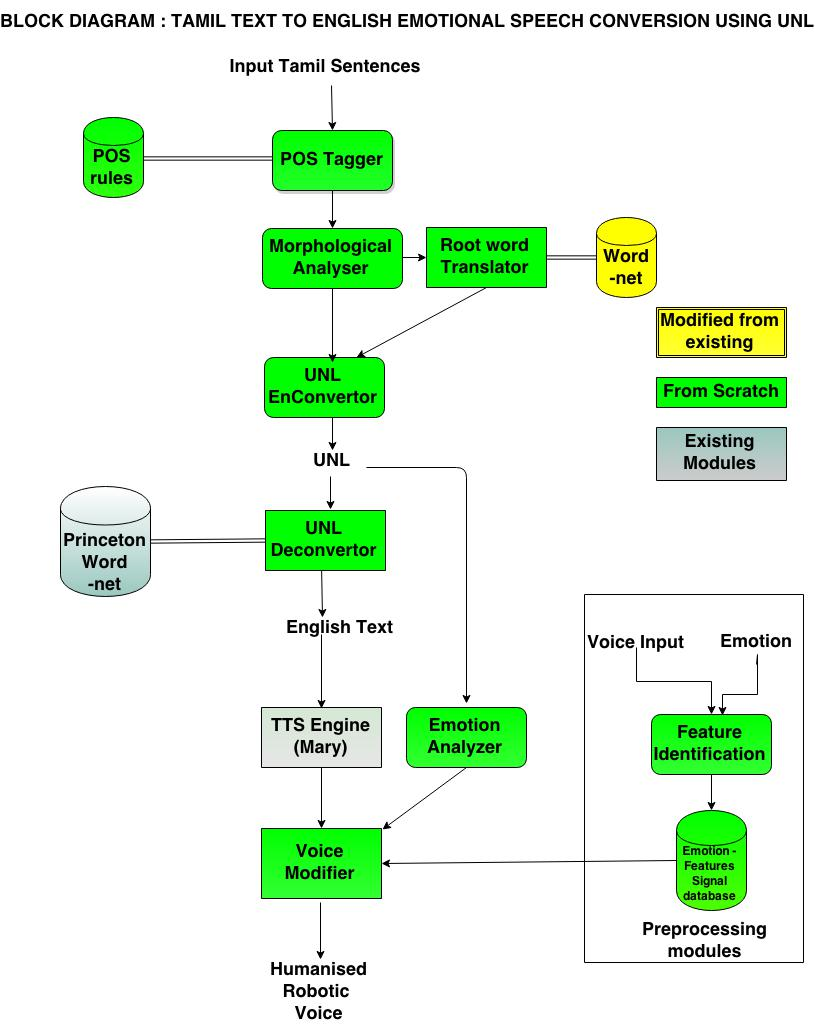
\includegraphics[width=\textwidth]{block}
\section{Description of Input and Output}\large
\begin{center}
\begin{tabularx}{\linewidth}{|@{}lYYYYY@{}|}
\hline\hline
MODULES & INPUT & OUTPUT\\
\hline
POS Tagger & 
\end {tabularx}
\end{center}

\section{Evaluation Parameters for Modules}\large
\begin{center}
\begin{tabularx}{\linewidth}{|@{}lYYYYY@{}|}
\hline
MODULES & EVALUATION PARAMETERS \\ 
\hline\hline
	POS Tagger &  Output from existing tagger - Kadhambam\\
\hline
Morphological Analyser & Output from existing analyers - Atcharam\\
\hline
	Emotion-features signal database construction
& \begin{itemize}
\item The number of variations between the values of F0 determined in time domain and frequency domain.
\item The number of values of F0 that are harmonics i.e, multiples of fundamental frequency F0
\end{itemize}\\
\hline
	Emotion identification & 
\begin{itemize}
\item The number of times the correct emotion is identified.
\item The number of times the appropriate degree of the emotion is identified.
\end{itemize}\\
\hline
	Voice Modification and Output &
\begin{itemize}
\item Using a public poll to determine, on a scale from 1 to 5 how emotional the final output is.
\item A poll to determine what emotion is expressed by the output 
\item Number of times an emotion is correctly recognized. 
\item Number of times an emotion is wrongly recognized.
\end{itemize}
\end {tabularx}
\end{center}

\end{document}
